\chapter{Selection and development}
\label{Selection}

This chapter covers the package selection and the setup of all nodes in the concept. In addition to that the development of the custom nodes will be discussed. This results in nodes assigned to each block in the schematic pictured in Figure \ref{navconcept}.


\section{Simulation}
There are many options, when it comes to robot simulation environments, which makes a proper selection mandatory. The chosen simulator then needs to be configured and equipped with models, sensors and a drive system.

\subsection{Selection}
To begin of the selection process a group of reasonable simulators needs to be collected. The two selected options are Gazebo and V-REP since they are the two most used robotics 3D simulators \cite{SimComp}.\\
The newest version of V-Rep is now called CoppeliaSim. Unfortunately, there are no comparisons between it and Gazebo yet. Performing a thorough comparison between both would exceed the scope of this thesis. Therefore, its predecessor V-Rep will be compared. \\

Both simulators seem to fulfill most of the defined requirements to a certain extend, while Gazebo seems to have a easier installation process and integration into ROS.\\
Gazebo is included in the default packages of ROS Noetic since it is developed by the Open Source Robotics Foundation as the default simulator for ROS\cite{ROSPkg}.

V-REP, as well as Gazebo, offers plugins and URDF conversion for custom models, but an even bigger selection of mobile robot models. Unfortunately, they can only be used as examples since the required models are very specific.\\
In contrast to V-REP, Gazebo does not contain an integrated model editor.

The comparison in the paper of L. Pitonakova et al. regarding computational load shows, that V-Rep is the most resource hungry environment, when compared to  Gazebo\cite{Pitonakova}. Real time simulation is highly wanted in this thesis, so the results can be compared to real results in the future.

Based on the fact, that Gazebo is included in the ROS-Noetic package list and has a smaller computational load compared to V-Rep, it will be the simulation environment in this project.

\subsection{Model}
Since Gazebo doesn't have an integrated model editor the freeware ``Blender'' will be used for the generation of the model of the environment, since it has options for exporting COLLADA files (.dae) usable in Gazebo.

As described in the requirements the robot models will be generated using URDF which will be covered later.

\section{move\_base}

As described in the concept, the navigation stack will be used in this thesis. Therefore, the action move\_base will be used to get the robot to a given goal.\\
 move\_base incorporates nav\_core and costmap\_2d and their internal nodes, which need to be selected according to the requirements of the navigation.\\
Similar to the separation described in the concept (chapter \ref{concept})the nodes will be categorized into a global and local stage and discussed individually.

\subsection{Global stage}
\label{globalconfig}
\subsubsection{Planner}

Since the global planner needs to communicate with the nav\_core interface  the following selection as described in the documentation of nav\_core can be used as possible candidates\cite{navcore}:

\begin{itemize}
	\item global\_planner
	\item navfn
	\item carrot\_planner
\end{itemize}


Here the choice is fairly easy, since base\_global\_planner is the successor of navfn. It still supports the the behavior of navfn, but it offers more options, such as A* planning algorithm instead of Dijkstra.


carrot\_planner isn't suited for this use-case since it doesn't fullfil the requirement of being able to cover lane changes since it will not generate plans, that go around obstacles. Instead it will generate a straight path to the goal and shortens the path if the goal is behind or in an obstacle\cite{corrotplanner}.

\subsubsection{Costmap}
Since costmap\_2d is embedded in move\_base the package does not need to be selected itself. Instead the layers of the individual costmap need to be selected.\\

As defined in the concept, the global costmap needs to have information about lethal obstacles, road markings, as well as a defined preference for the right lane.\\


The data, supplied by the lidar and the road detection, can be marked as lethal obstacles in the costmap using the obstacle layer. This data consist solely from points, meaning there are gaps between the individual measurements. In the case of the lidar, these size of these gaps increase with the measurement distance.\\

As soon as these gaps are larger than the resolution of the costmap, free cells will start to appear between the measurements, that allow the planner to generate paths through obstacles or the road markings.\\

To solve this issue the default layer ``inflation\_layer'' can be used. This layer inflates every lethal cell in the costmap by a fixed radius, closing the previously discussed gaps like pictured in figure \ref{costinfl}.\\

\begin{figure}[H]
	\centering
	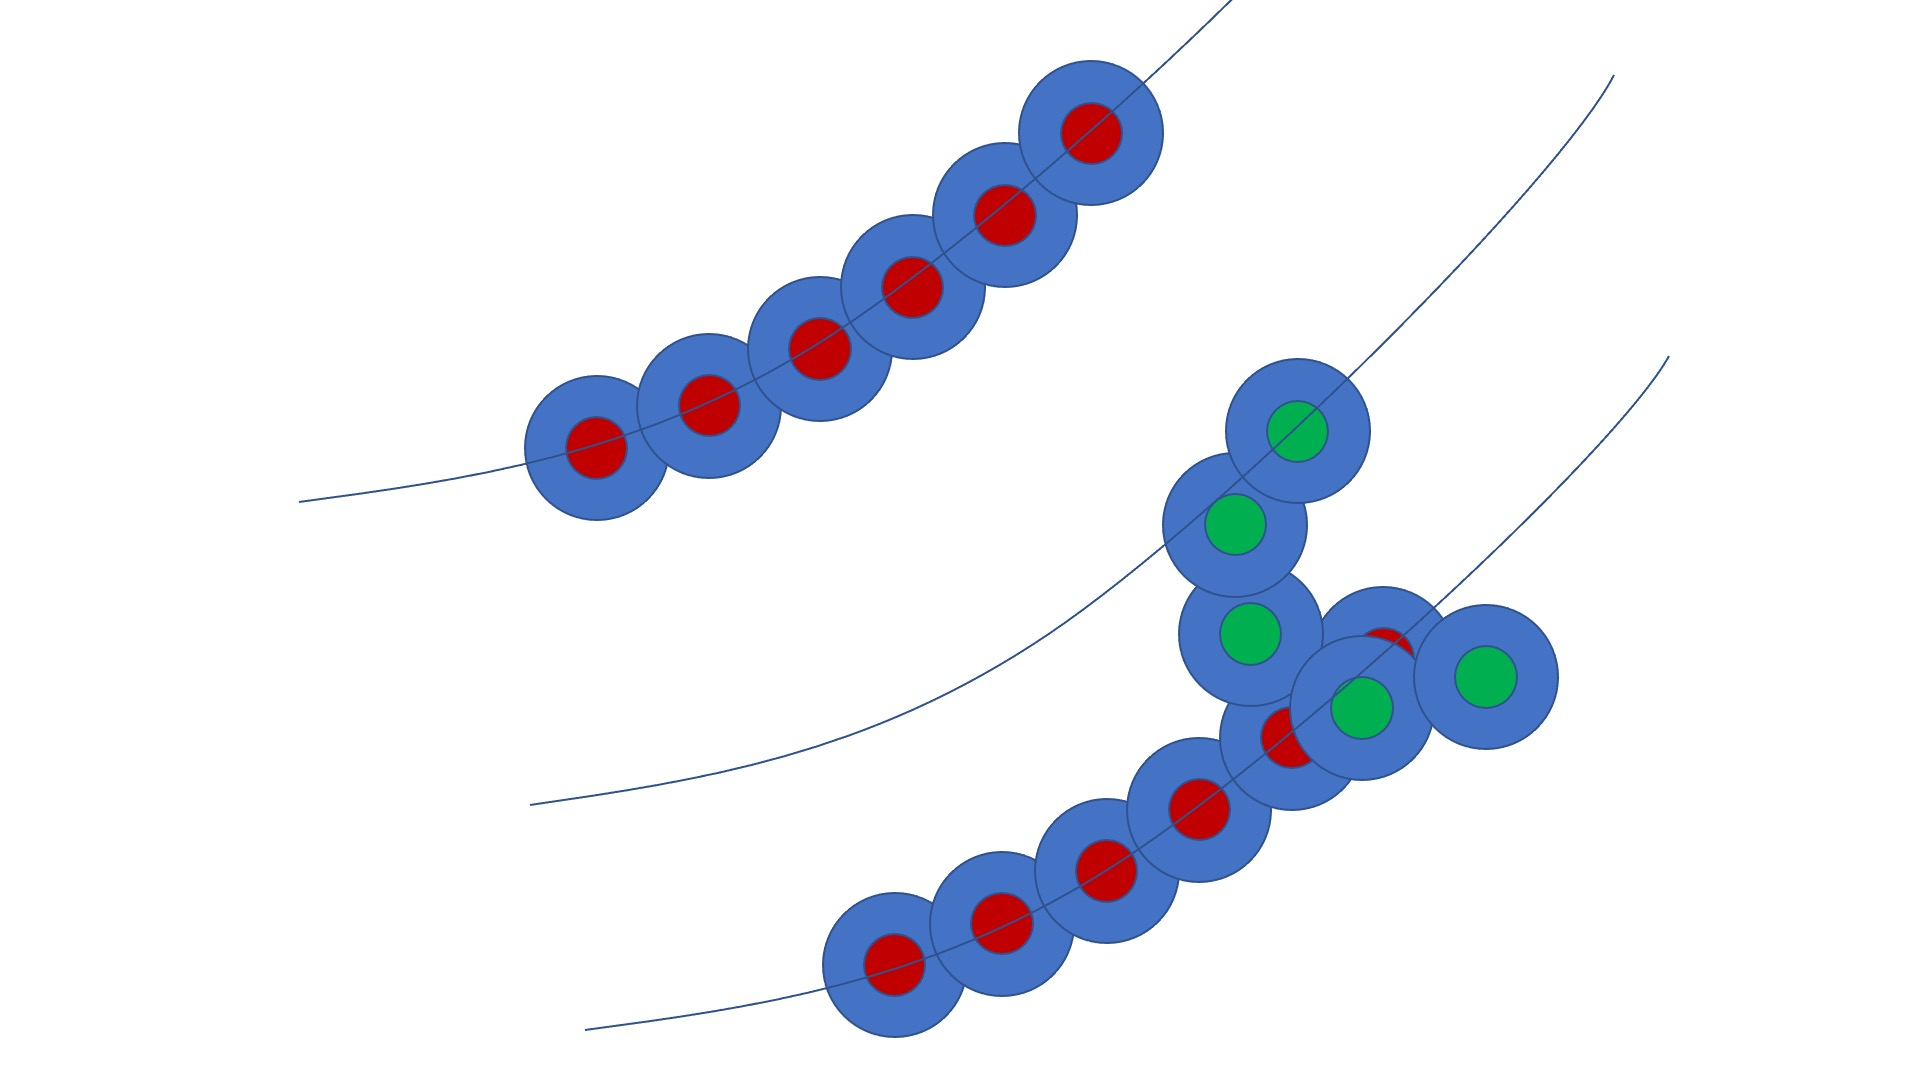
\includegraphics[width=.7\textwidth]{Pictures/costmap inflation}
	\caption{visualization of the inflated sensor data in the costmap (red - road detection, green - lidar scan, blue - inflation)}
	\label{costinfl}
\end{figure}

This configuration allows the navigation to plan around obstacles, without leaving the road, but there is no preference for the right lane yet. To generate this preference the left lane has to have higher cost than the right lane, without being lethal.

Unfortunately, this can not be solved using the provided layers. Therefore a custom layer has to be developed.

The only information about where the lane is, comes from the road detection, which outputs polynomials that approximate the road markings. The aim is to make a gradually increasing cost from the middle of the right lane to the left road marking. Therefore, the left road marking needs to be inflated using dynamically adjustable parameters for the cost distribution.\\


To guarantee, that driving on the right lane, the right road marking will be inflated, but with a different cost distribution. Here only the road marking is lethal, whereas the lane should be free resulting in the cross section pictured in \ref{globalcostdistro}. To simplify lane changes in the case of obstacle avoidance these obstacles need to have a cost free zone around them.\\

The layer should also feature a reset option as a recovery behavior.

\begin{figure}[H]
	\centering
	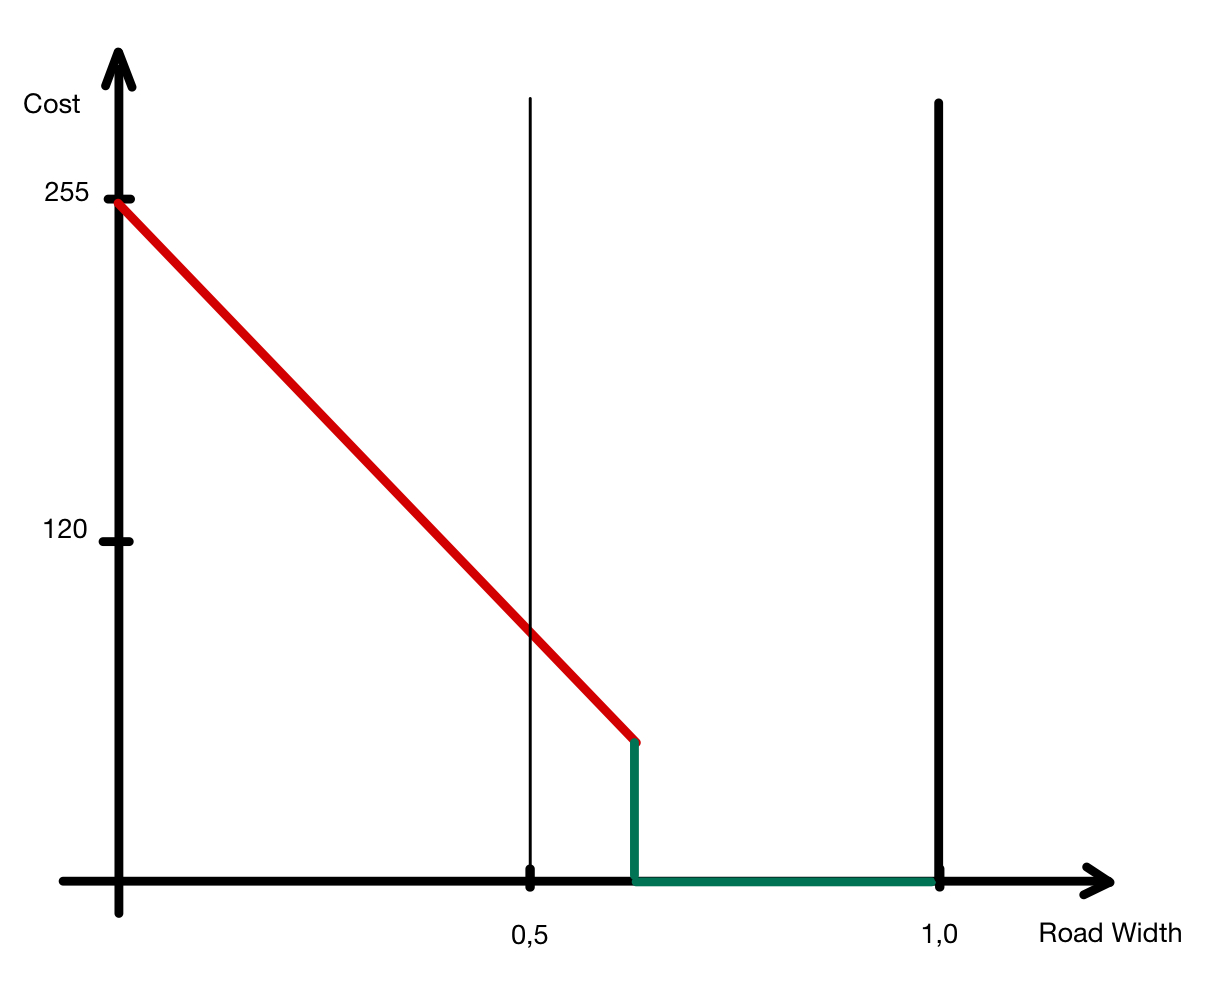
\includegraphics[width=.8\textwidth]{Pictures/global stage cost distro}
	\caption{global costmap cross section of the road}
	\label{globalcostdistro}
\end{figure}



The previously discussed tasks for the layer can be summarized in the following requirements:

\begin{itemize}
	\item Input for points
	\item Input of point individual inflation parameters
	\item Rasterization of the individual cost distribution
	\item Service to reset the cost in the layer
\end{itemize}



\subsection{Local stage}
\subsubsection{Planner}
In contrast to the global planner there are way more options for the local planner node to choose from. Like the global planners the local planners will be selected using the options offered in the following description of nav\_core\cite{navcore}.

\begin{itemize}
	\item base\_local\_planner
	\item dwa\_local\_planner
	\item eband\_local\_planner
	\item teb\_local\_planner
	\item mpc\_local\_planner
\end{itemize}

To choose the local planner the requirements have to be defined first.\\

Since the global planner is taking care of the obstacles and the road lanes, the local planner has the general task of following the global path and creating a command velocity that is feasible in regards to the dynamics of the robot.\\

Smooth lane changes are highly wanted in this project. This will help the camera and therefore the road detection to keep seeing the road during a lane swap. To achieve this, the planner is supposed to drive close to the global plan and to smooth out the edges.
Furthermore the local planner needs to have a good performance in tight corridor situations, since those will often be caused by obstacles blocking one lane.\\

During all of this the local planner needs to use the information of lethal obstacles to prevent crashes in its optimized path.\\


Base and DWA are two planners that are included in the navigation stack. Similar to the global planner selection, the successor and therefore DWA is chosen seems like a good option. According to Kaiyu Zeng, this is the general recommendation for mobile robotics platforms\cite{navtuningguide}. As described in the theoretical background, dwa struggles with navigation in narrow corridors and therefore can not be used.

In contrast to the method of the dwa planner, the elastic band approach is better suited for narrow corridors. The two planner, that use this approach are eband\_local\_planner and teb\_local\_planner. Choosing between these two is difficult, since they both share the same base principle. teb\_local\_planner is better suited for this use case, since it supports both car like and differential robots.

mpc\_local\_planner is build using the popular model predictive control approach. According to Christoph Rösmann (the developer of both planners), teb is preferred when dealing with simple differential or car like robots\cite{mpcvsteb}. 

According to the previous analysis teb\_local\_planner has the best fit to the use case and therefore selected for the navigation.


\subsubsection{Costmap}
The local planner is only supposed to generate velocity commands that lead to no lethal collision. Therefore, the local costmap will have the same layers as the global one without the dynamic inflation layer that is used to guide the robot to the right lane.


\section{PoseFinder}
As described in the concept the purpose of this node is to determine the pose of the next goal and send it to the move\_base action client. Therefore, it will need to process the data from the road detection and if available from the SLAM map to determine a feasible goal.\\

Since the robot should never reach a goal, the PoseFinder needs to determine new goals at a configurable frequency. 

\subsection{Usage of Current Camera Data}


The easiest way to get new goals, is to take the last point of the polynomial provided by the road detection as the position and calculate the yaw angle of the new goal with the gradient of the last two points.\\

While this is a logical approach in an ideal scenario, it certainly will not work in a realistic one, since a continuous data stream from the road detection can not be guaranteed, as shown in the edge cases pictured in figure \ref{nav edge case}.\\

In all examples pictured in figure \ref{nav edge case}, the road detection is not able to detect the road. If the robot would only follow the lanes detected by the road detection, it would not be able navigate in these situations, leading to stop of the robot.\\

This introduces the requirement for the PoseFinder, to find goals by estimating the course of the road, based on the latest data of the road detection. Therefore the navigation bridges the gap, in which the camera can not see the road.\\

\begin{figure}
	\centering
	\begin{subfigure}{.24\linewidth}
		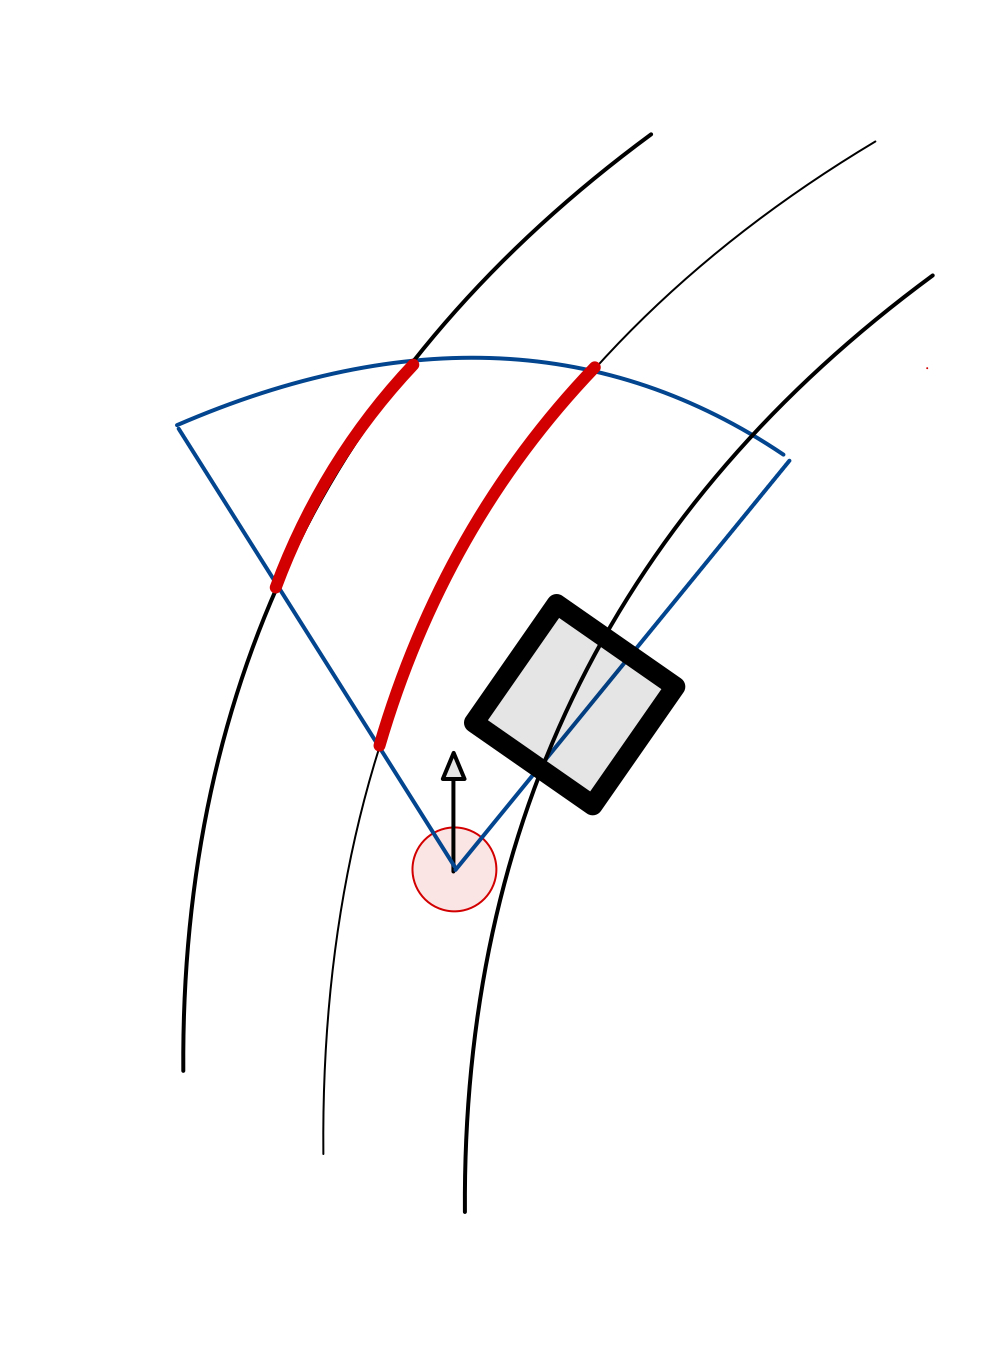
\includegraphics[width=\textwidth]{Pictures/road detection obstacle}
		
		\caption{lane markings blocked by obstacle}
	\end{subfigure}
	%\hskip2em
	\begin{subfigure}{.24\linewidth}
		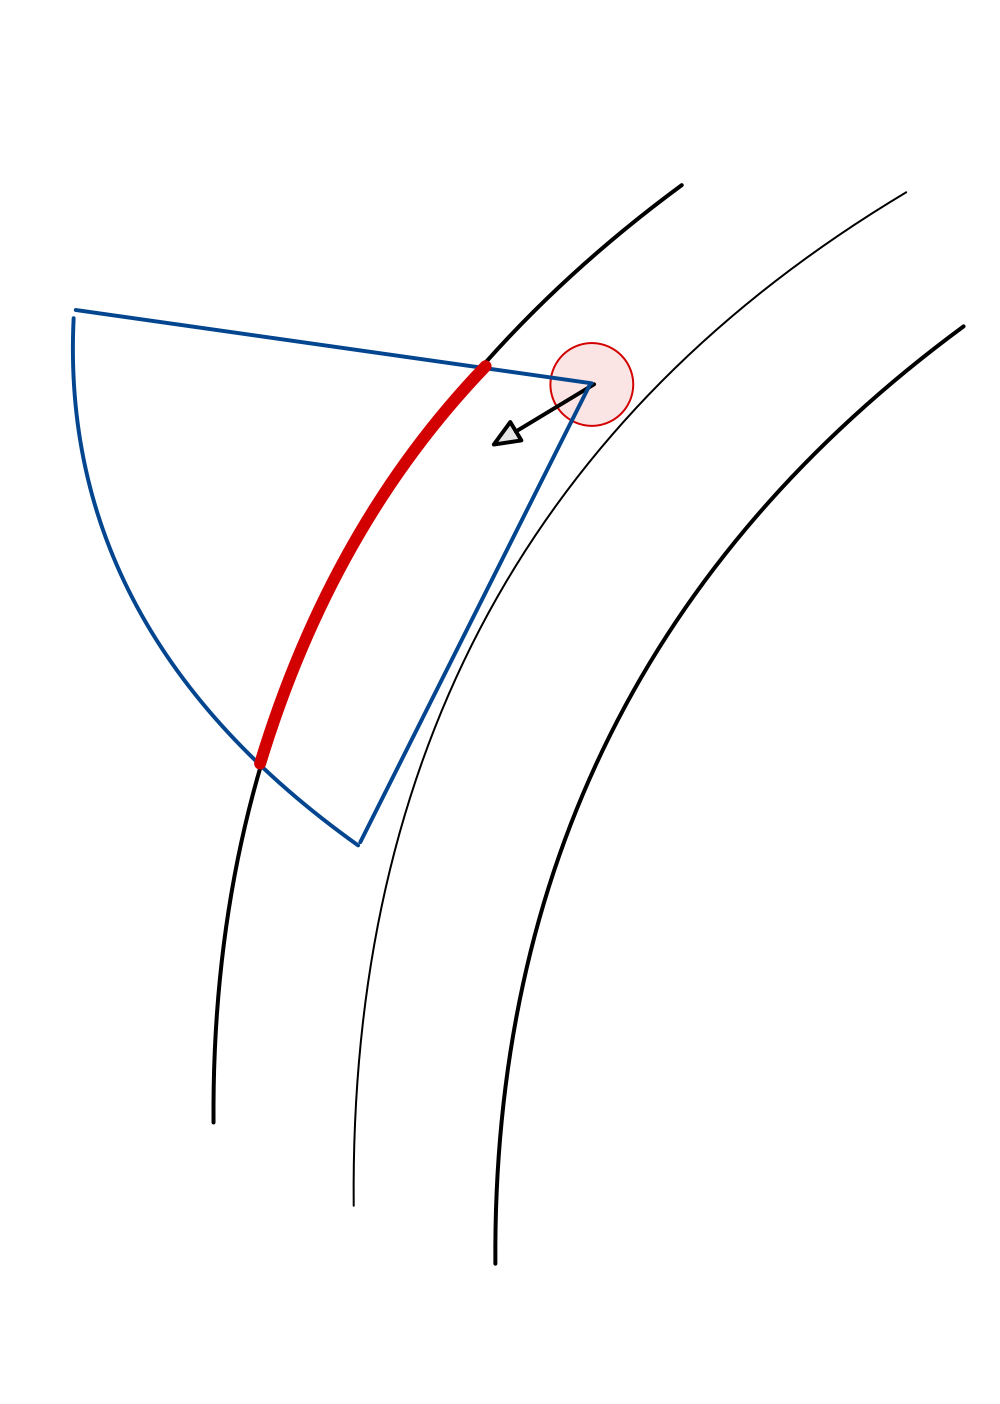
\includegraphics[width=\textwidth]{Pictures/road detection angle}
		\caption{driving in a corner}
	\end{subfigure}	
	%\hskip2em
	\begin{subfigure}{.24\linewidth}
		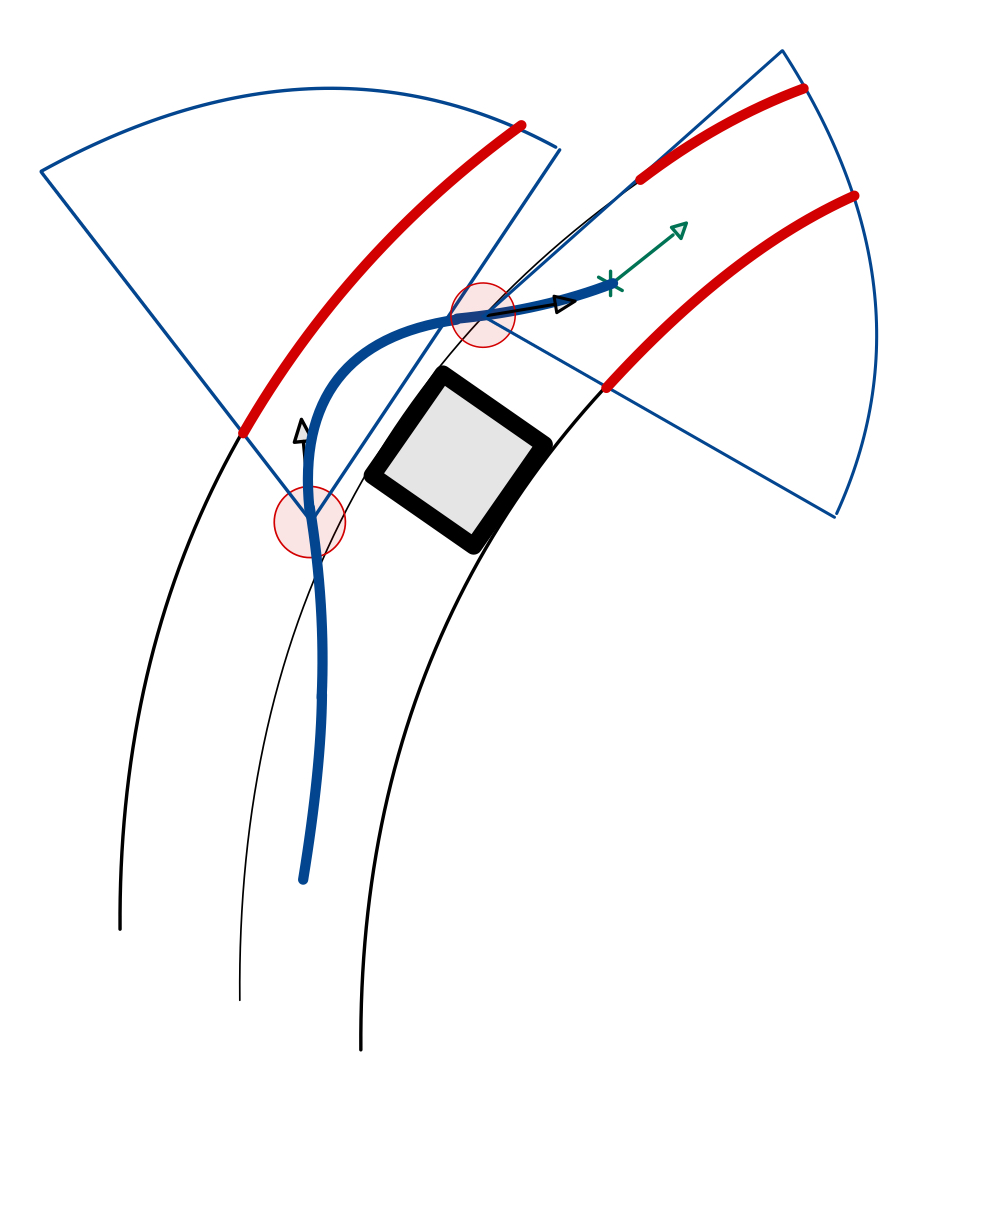
\includegraphics[width=\textwidth]{Pictures/road detection blind}
		\caption{camera angle during avoidance}
	\end{subfigure}
		%\hskip2em
	\begin{subfigure}{.24\linewidth}
		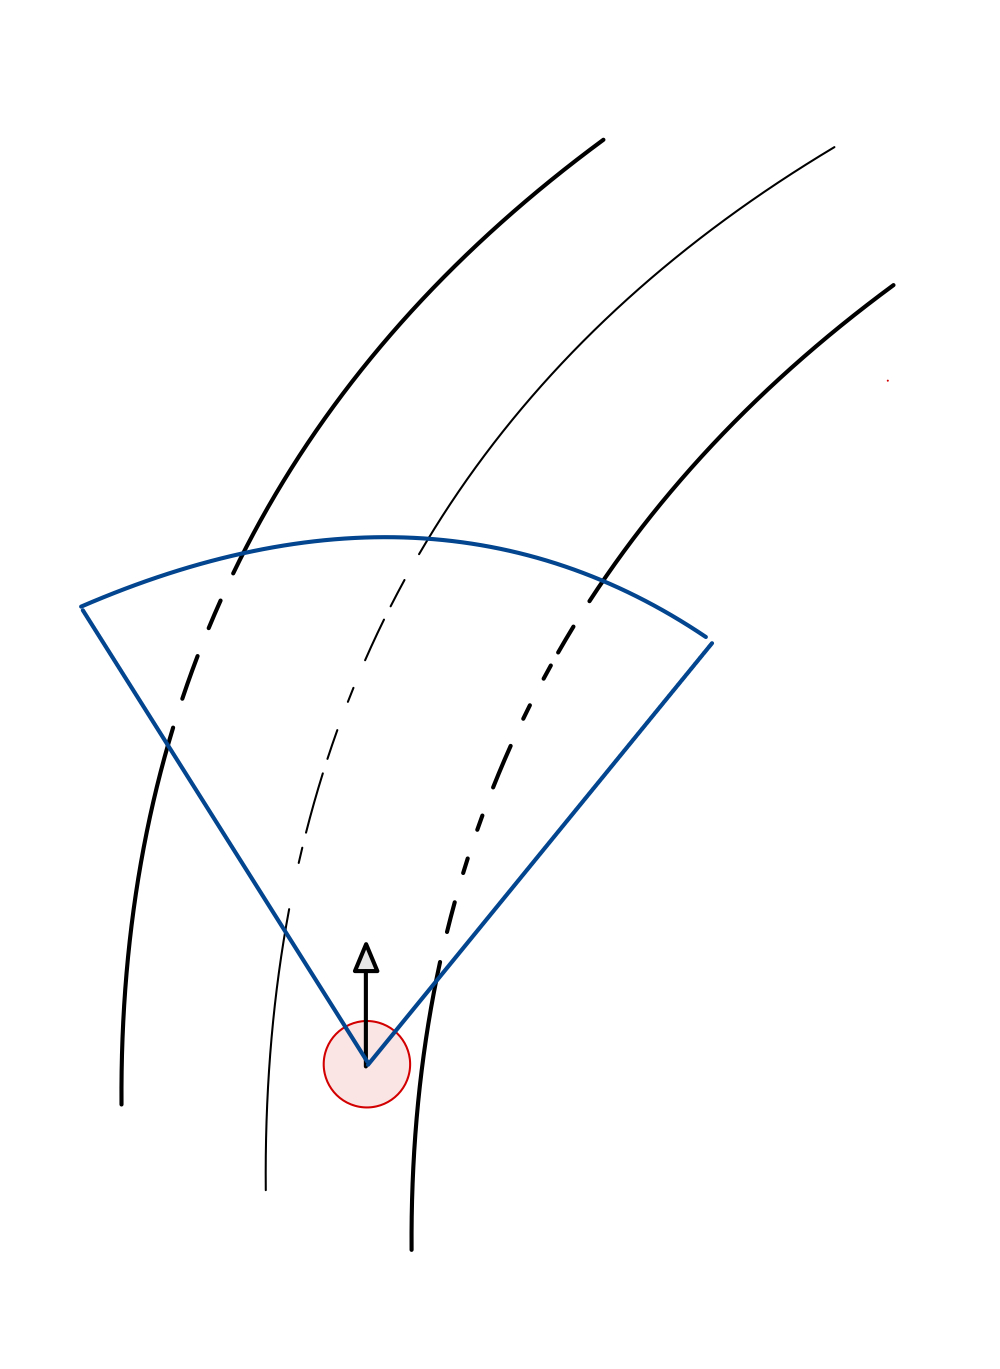
\includegraphics[width=\textwidth]{Pictures/road detection noise}
		
		\caption{camera noise or bad road markings}
	\end{subfigure}


	\caption{edge cases that prevent simple lane following}
	\label{nav edge case}
\end{figure}



\subsection{Approximations}
\label{aprox}
The approximation provided by the road detection is in the form of a polynomial. These describe the real road very accurately, but only in a very restricted domain. Outside of this domain, these polynomials diverge rapidly from the real road, making them unusable for any estmates.

Since the road mostly consists of circles of varying radii and origins, it is self evident, that using the polynomials in their restricted domain to represent a section of a circle will give a better estimate.\\
This circle can be calculated using the least square approach presented in Randy Bullocks paper on least square circle fitting \cite{leastsquarecircle}.\\

In theory this approximation should work for nearly straight sections as well. This will cause radius and origin to trend to infinity. Caused by camera noise and the inaccuracy of the road detection the representation of straight sections will get increasingly inaccurate.\\

Similar to the least square approach for circles, an approach for the lines can be formulated.

Switching between the result of the two approximations will produce the best result for both scenarios. This switching will be triggered by the radii of the approximated circles exceeding a configurable threshold.\\

The next step is a goal extraction from the chosen approximation. This goal will be calculated at a given distance from the robot origin on the approximated route. In contrast to the approximated lines, the circles have a defined angle of trustworthiness. Otherwise small circles would cause the goal to be way of the prediction. The orientation of the goal will then be determined using the derivative of either, the approximated circles or lines.\\

With the calculated points on both circles or on both lines the mean can be calculated and represents the new goal for the robot.

\begin{figure}[H]
	\centering
	\begin{subfigure}{.45\linewidth}
		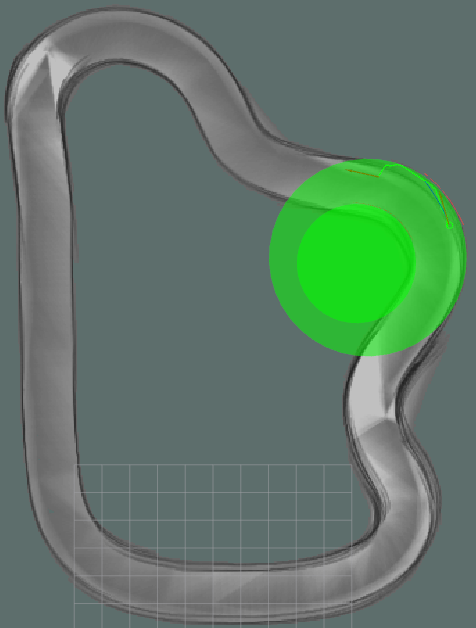
\includegraphics[width=\textwidth]{Pictures/circle approx}
		\caption{circle approximation}
		\end{subfigure}	
	%\hskip2em
	\begin{subfigure}{.45\linewidth}
		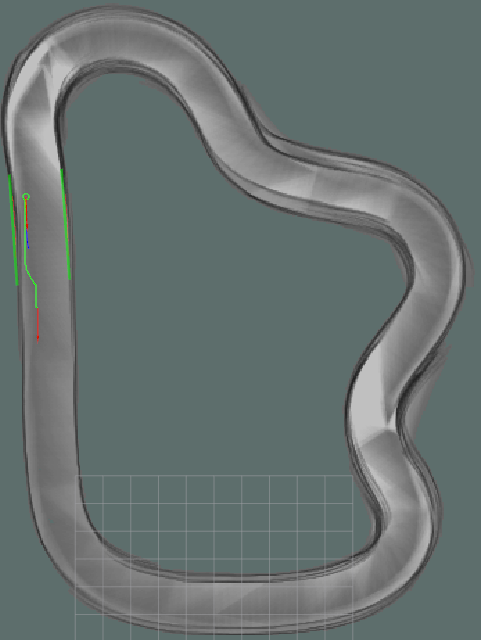
\includegraphics[width=\textwidth]{Pictures/lineapprox}
		\caption{line approximation}
	\end{subfigure}

	\caption{Approximations visualizations}
	\label{aproxvis}

\end{figure}

A visualization of the result is pictured in figure \ref{aproxvis}.
It shows the robot, its current goal, as well as the estimated road outlined by the geometric shapes of the respective approximation.

Based on this figure the necessity of the angle of trustworthiness of the road detection becomes apparent. Assuming a larger goal distance the estimated goal would not be located on the road anymore and would point in the wrong direction as well. This makes pathfinding impossible without leaving the road.


While these approximations allow the robot to bridge the edge cases pictured in \ref{nav edge case}, this approach introduces new problems. Since the goal is now determined by using estimations, it is uncertain if the goal is located off the road, or even in an obstacle. This problem is pictured in figure \ref{goaluncertainty}. Here the goal of the navigation is located within an obstacle. This would make path finding to the goal impossible.\\

To solve this issue the navigation has to consider obstacles, only if they are significantly closer to the robot than the goal. Therefore, the navigation treats the road as ``free'' until the obstacle is close to the robot. At this moment the predicted goal is way behind the obstacle, leading to an avoidance as described in the requirements of the navigation.

This does not only affect the distance, at which the PoseFinder estimates goals, but also the distance at which obstacles are treated as such and marked in the costmap, which has to be considered during the configuration.

\begin{figure}
\centering
	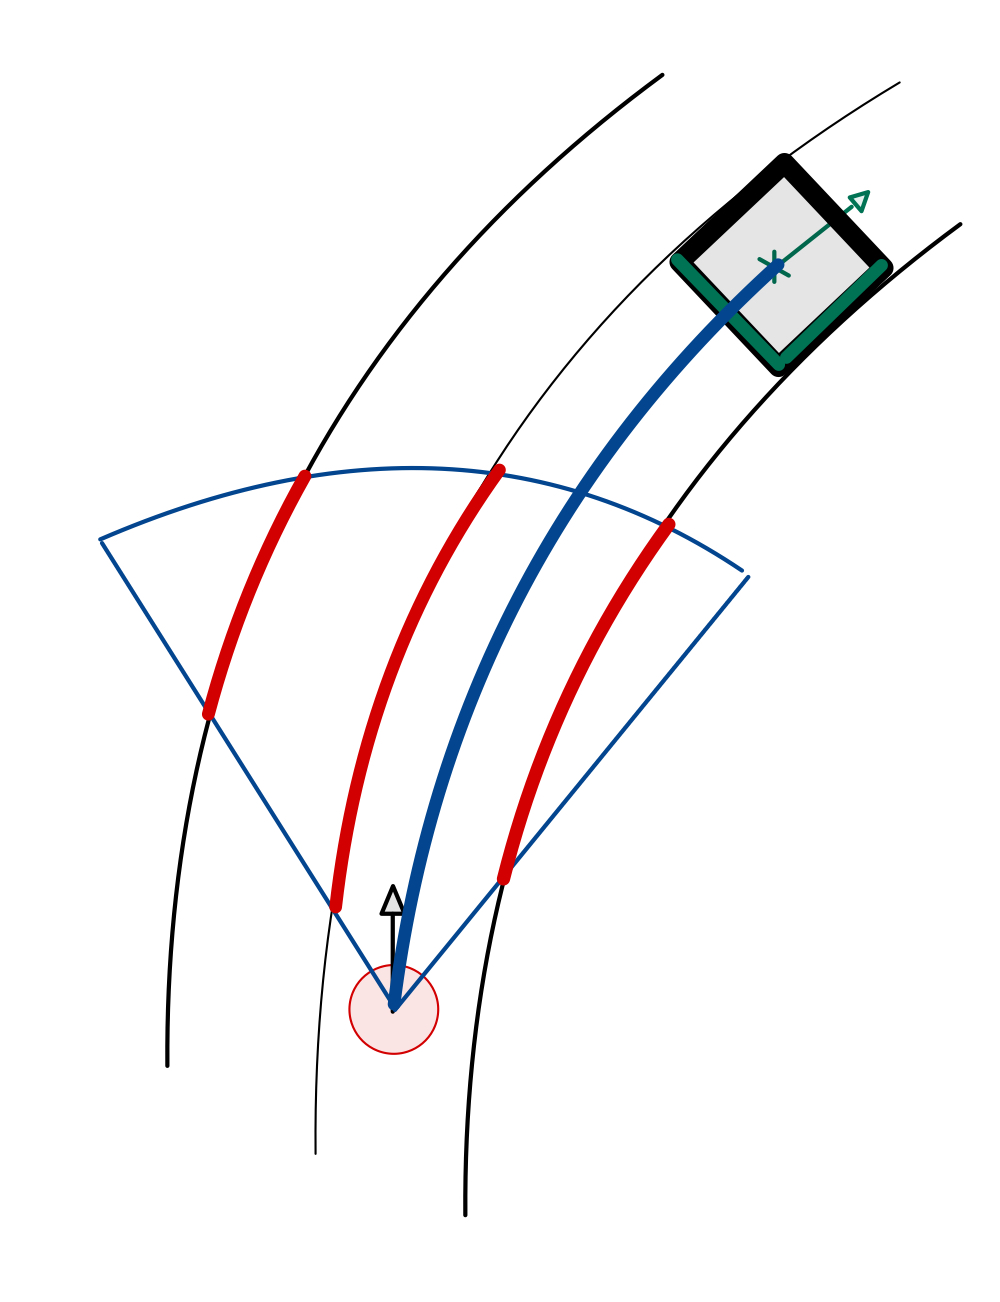
\includegraphics[width=0.33\textwidth]{Pictures/finding goal in obstacle}
	\caption{uncertainty of predicted goals }
	\label{goaluncertainty}
\end{figure}


\subsection{Goal from map}

If the robot is running a SLAM algorithm during the first round, the goal can be extracted directly from the SLAM map afterwards. This is more efficient and provides goals that will always be on the road. Furthermore the distance, at which goals will be found can be increased, this results in higher speeds of the robot and/or lower planner frequencies.\\

To find a goal in the SLAM map a circle rasterization algorithm will be used, based on Bresenham rasterization \cite{ComputerGraphics}.\\

This algorithm finds every cell on a circular path around the robot and its associated value in the map. The values outside of a given FOV (field of view) can be eliminated. The remaining values with a larger likelihood than a configurable threshold will be reduced to one point by taking the mean value of them.\\

The orientation of the goal is determined by using the previously explained approximation algorithms.

\subsection{Concept}

Based on the previously proposed ways to determine goals, the concept pictured in figure \ref{posefinder structure} can be deduced.\\

\begin{figure}[H]
	\centering
	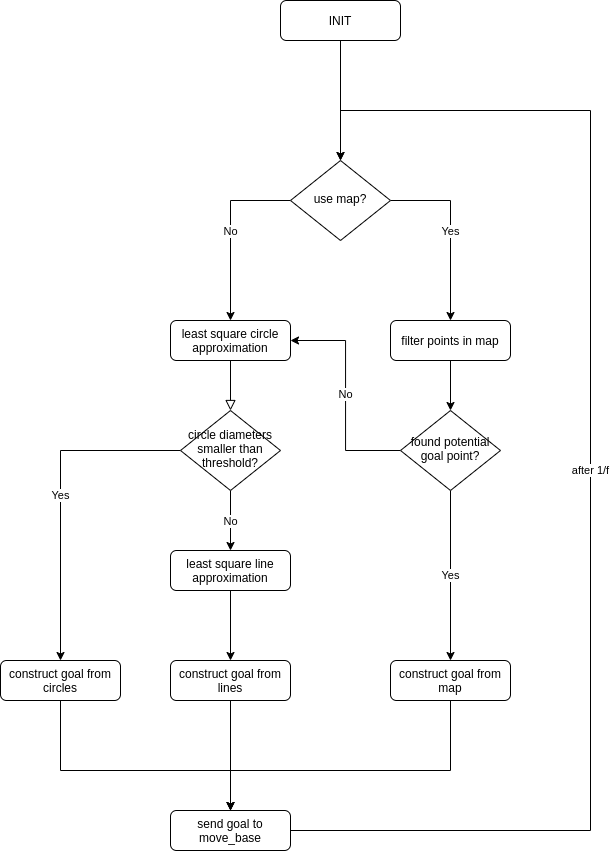
\includegraphics[width=.9\textwidth]{Pictures/posefinder diagram}
	\caption{PoseFinder internal structure}
	\label{posefinder structure}
\end{figure}

The goalfinding algorithms are ordered based on their expected accuracy.

An accurate map of the surrounding offers the best potential to find feasible goals on the upcoming road. Hence, it has to be checked first, if a goal can or should be extracted from the map.

As described, every section can be expressed by a circle segment. This approximation will have a higher priority than the line approximation.

Finally the line approximation will be checked and only, if the circle approximation generated circles with radii, that exceed a threshold for their trustworthiness.

The result of the chosen algorithm can be used to determine a goal that will be sent as an input to move\_base.

The goal found by the approximation, unfortunately is not certainly on the road. It could as well be in an obstacle or of the road, which would make complete navigation to the goal impossible. Hence this procedure will be repeated at a configurable frequency, so the robot will never reach one of the goals. 

The node is configurable using rqt\_reconfigure and the following parameters.

\begin{table}[H]
\centering
\resizebox{\columnwidth}{!}{%
\begin{tabular}{ l l l }
	
 \textbf{Parameter} & \textbf{Description} & \textbf{Range}\\
 cRadThresh & The Threshold for the radius of the circle approximation & 0.5-20 [m]\\ 
 goalDist & The maximum distance at which a goal should be found & 0.5-20 [m]\\  
 goalAngle & The maximum angle for the circle approximation higher priority than distance & 0.1-2 [$\pi$]\\  
 reductionRadius & Max distance at which points from the map will still be combined & 0.25-2.5 [m]\\  
 mapCostThresh & Threshold Cost Value for Map Data Extraction & 0-100\\  

\end{tabular}
}

\caption{PoseFinder parameters}
\label{posefinderparams}

\end{table}


\section{dynamic\_cost\_layer}
As described in the section \ref{globalconfig}, the global costmap requires a layer, that marks the left lane with increasing cost, to hinder the robot from leaving the right lane. This section builds upon the requirement definition in chapter \ref{Concept}.\\


To keep this layer flexible for other use cases, the generalized task of custom point inflation can be formulated. At first this seems similar to the inflation layer of the navigation stack, but the inflation layer inflates every lethal cell by one fixed distribution, whereas this layer is supposed to handle a custom distribution for every cell.\\

This behavior can be used to inflate the left road marking in the global costmap to force the global plan on the right side of the road, which is the behavior defined in the concept. The pluginis also supposed to be used to inflate cells with zero cost, which can be useful to guarantee a cost free right lane, or to give some free space around obstacles located on the road.\\


Figure \ref{dynnav} shows the cost zones generated by the dynamic\_inflation\_layer, and how the path finding algorithms could profit from this. The red sections are the ones with the actual cost distribution, whereas the blue and green sections are the zones, that are removed by the right road marking and the obstacle.\\

\begin{figure}
	\centering
	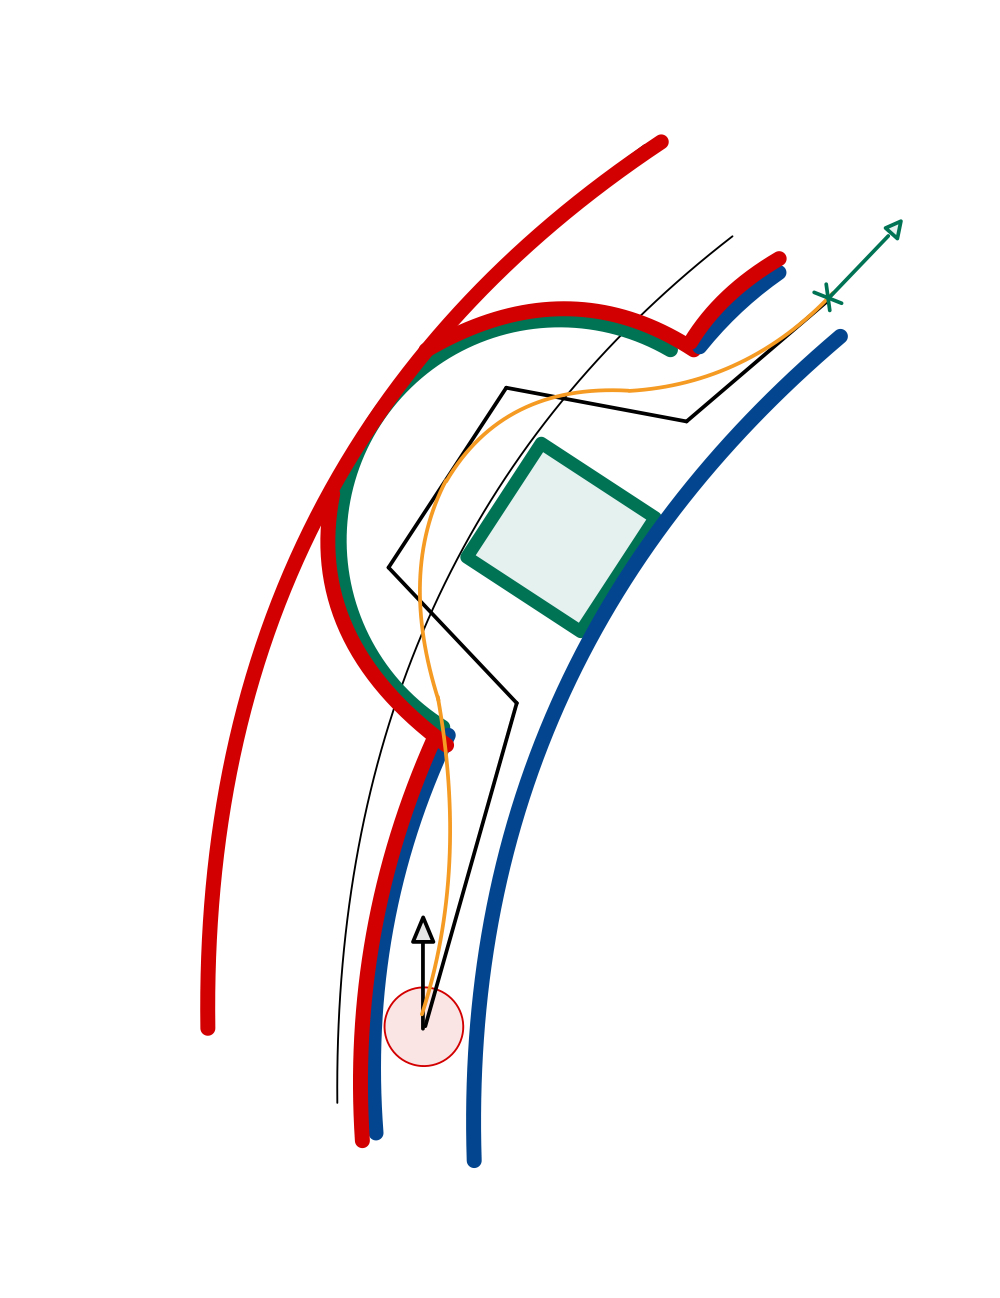
\includegraphics[width=.5\textwidth]{Pictures/inflationlayernav}
	\caption{navigation on road with dynamic\_cost\_layer}
	\label{dynnav}
\end{figure}


The layer receives a point cloud on a configurable topic. This point cloud is expected to feature channel values for the inflation radius, the maximum and the minimum cost for each individual point.\\

Since it can not be assumed, that the incoming points will be in the frame of the costmap the points in the costmap have to be transformed into the right frame using tf2.\\

Assuming a small resolution of the costmap and large inflation radii, the inflation algorithm has to compute and set a substantial amount of costs for each point of the point cloud. Therefore, efficiency is very important to being able to handle large point clouds in real time.\\

To minimize the computation load a Bresenham based algorithm for the circle rasterization will be used\cite{ComputerGraphics}. The point symmetry around the cell can be used to further minimize the computational load and only $\frac{1}{8}$th of the circle has to be computed. The rasterization process can be described by black cells on the perimeter of the circle in figure \ref{rasterization}.\\

\begin{figure}
	\centering
	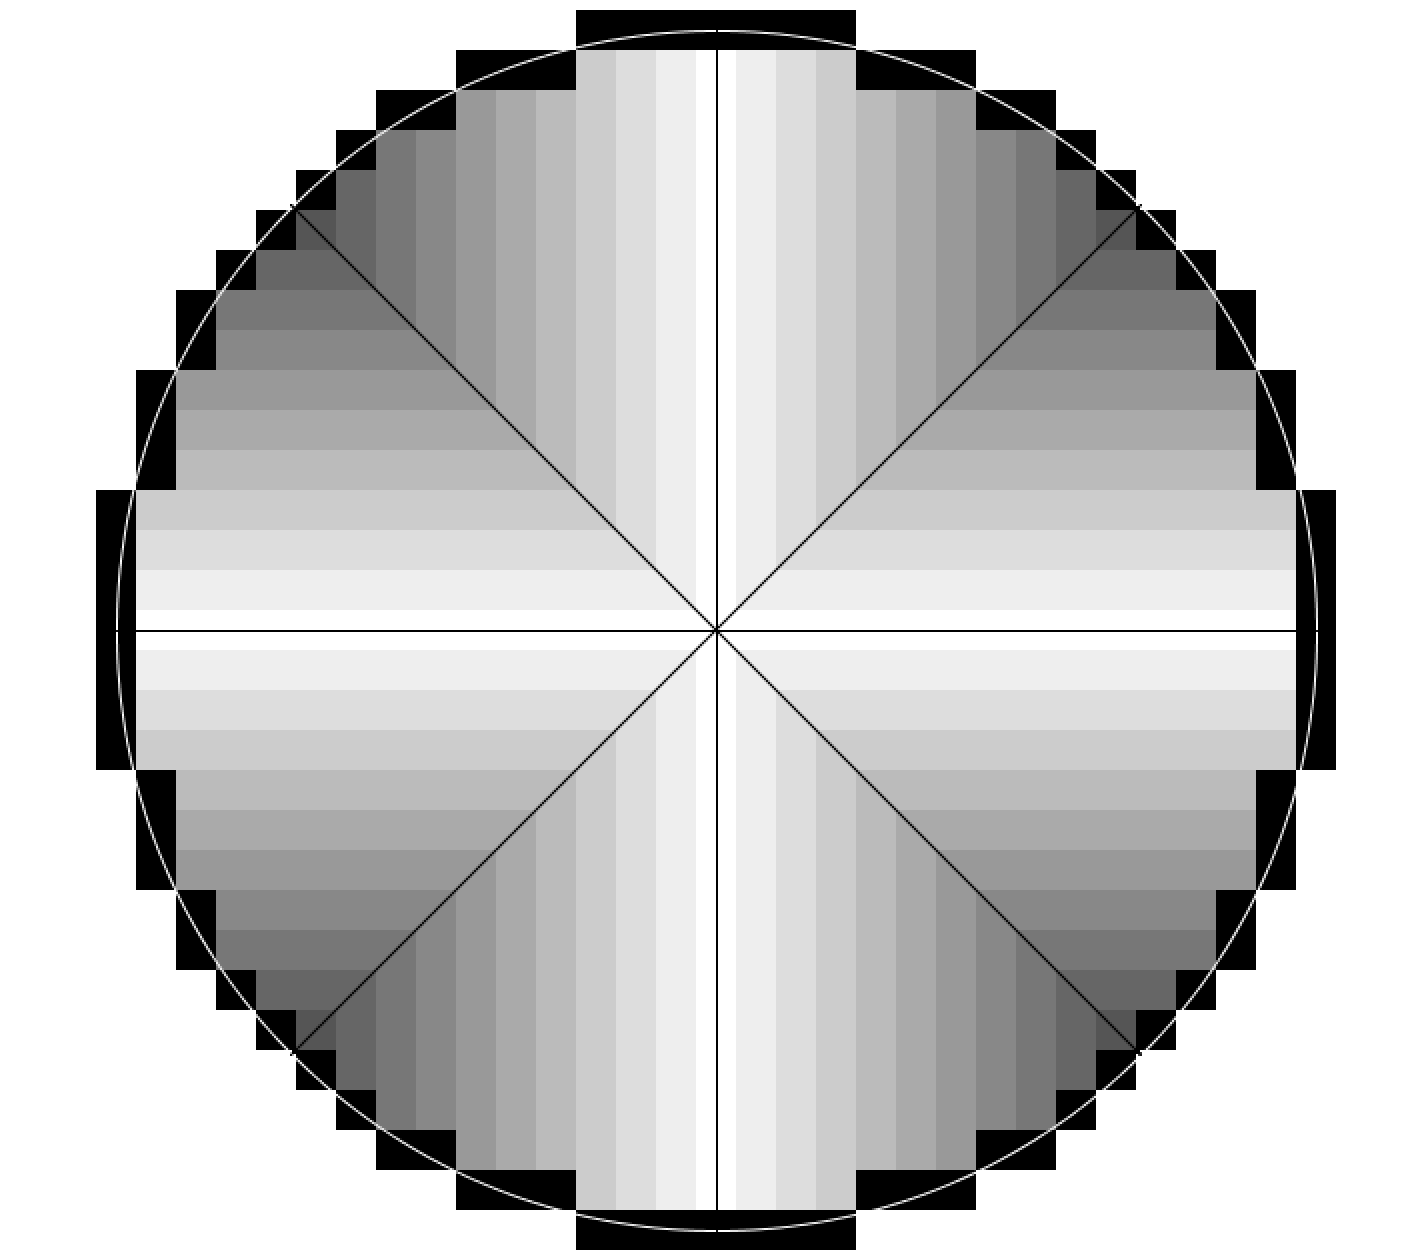
\includegraphics[width=.5\textwidth]{Pictures/rasterization}
	\caption{modified Bresenham rasterization with efficient surface filling}
	\label{rasterization}
\end{figure}


Adding to the typical behavior of the Bresenham rasterization the area of the circle will be filled using the point symmetry and by skipping overlapping points of the lines like in Figure \ref{rasterization}. Here it is visible, that every row with the same color is only calculated once and then projected in all eight octants. 
The cells within the circles perimeter are filled with the cost specified for that point. For this the following linear decaying \nth{1} degree function will be used which requires the computation of the distance of the rasterized cell to the center of the circle.

\[cost(distance)=maxcost-distance*\frac{maxcost-mincost}{radius}\]\\
with: \[distance=\sqrt{cell.x^2+cell.y^2}\]

 Since this will still require the usage of a square root for each cell in the circle This will be optimized as well.\\

The goal here is to use a function that contains only the squared distance and not many other mathematical operators, which still represents a decaying trend. This requirement rules out every function with an odd degree, all functions with an x offset and the normal distribution. This leaves all functions with an even degree from which the \nth{2} degree function is chosen to reduce square operators. The comparison between the two functions can be seen in the picture below.

\[cost(distance)=maxcost-distance^2*\frac{maxcost-mincost}{radius^2}\]\\

\begin{figure}[H]
	\begin{center}
	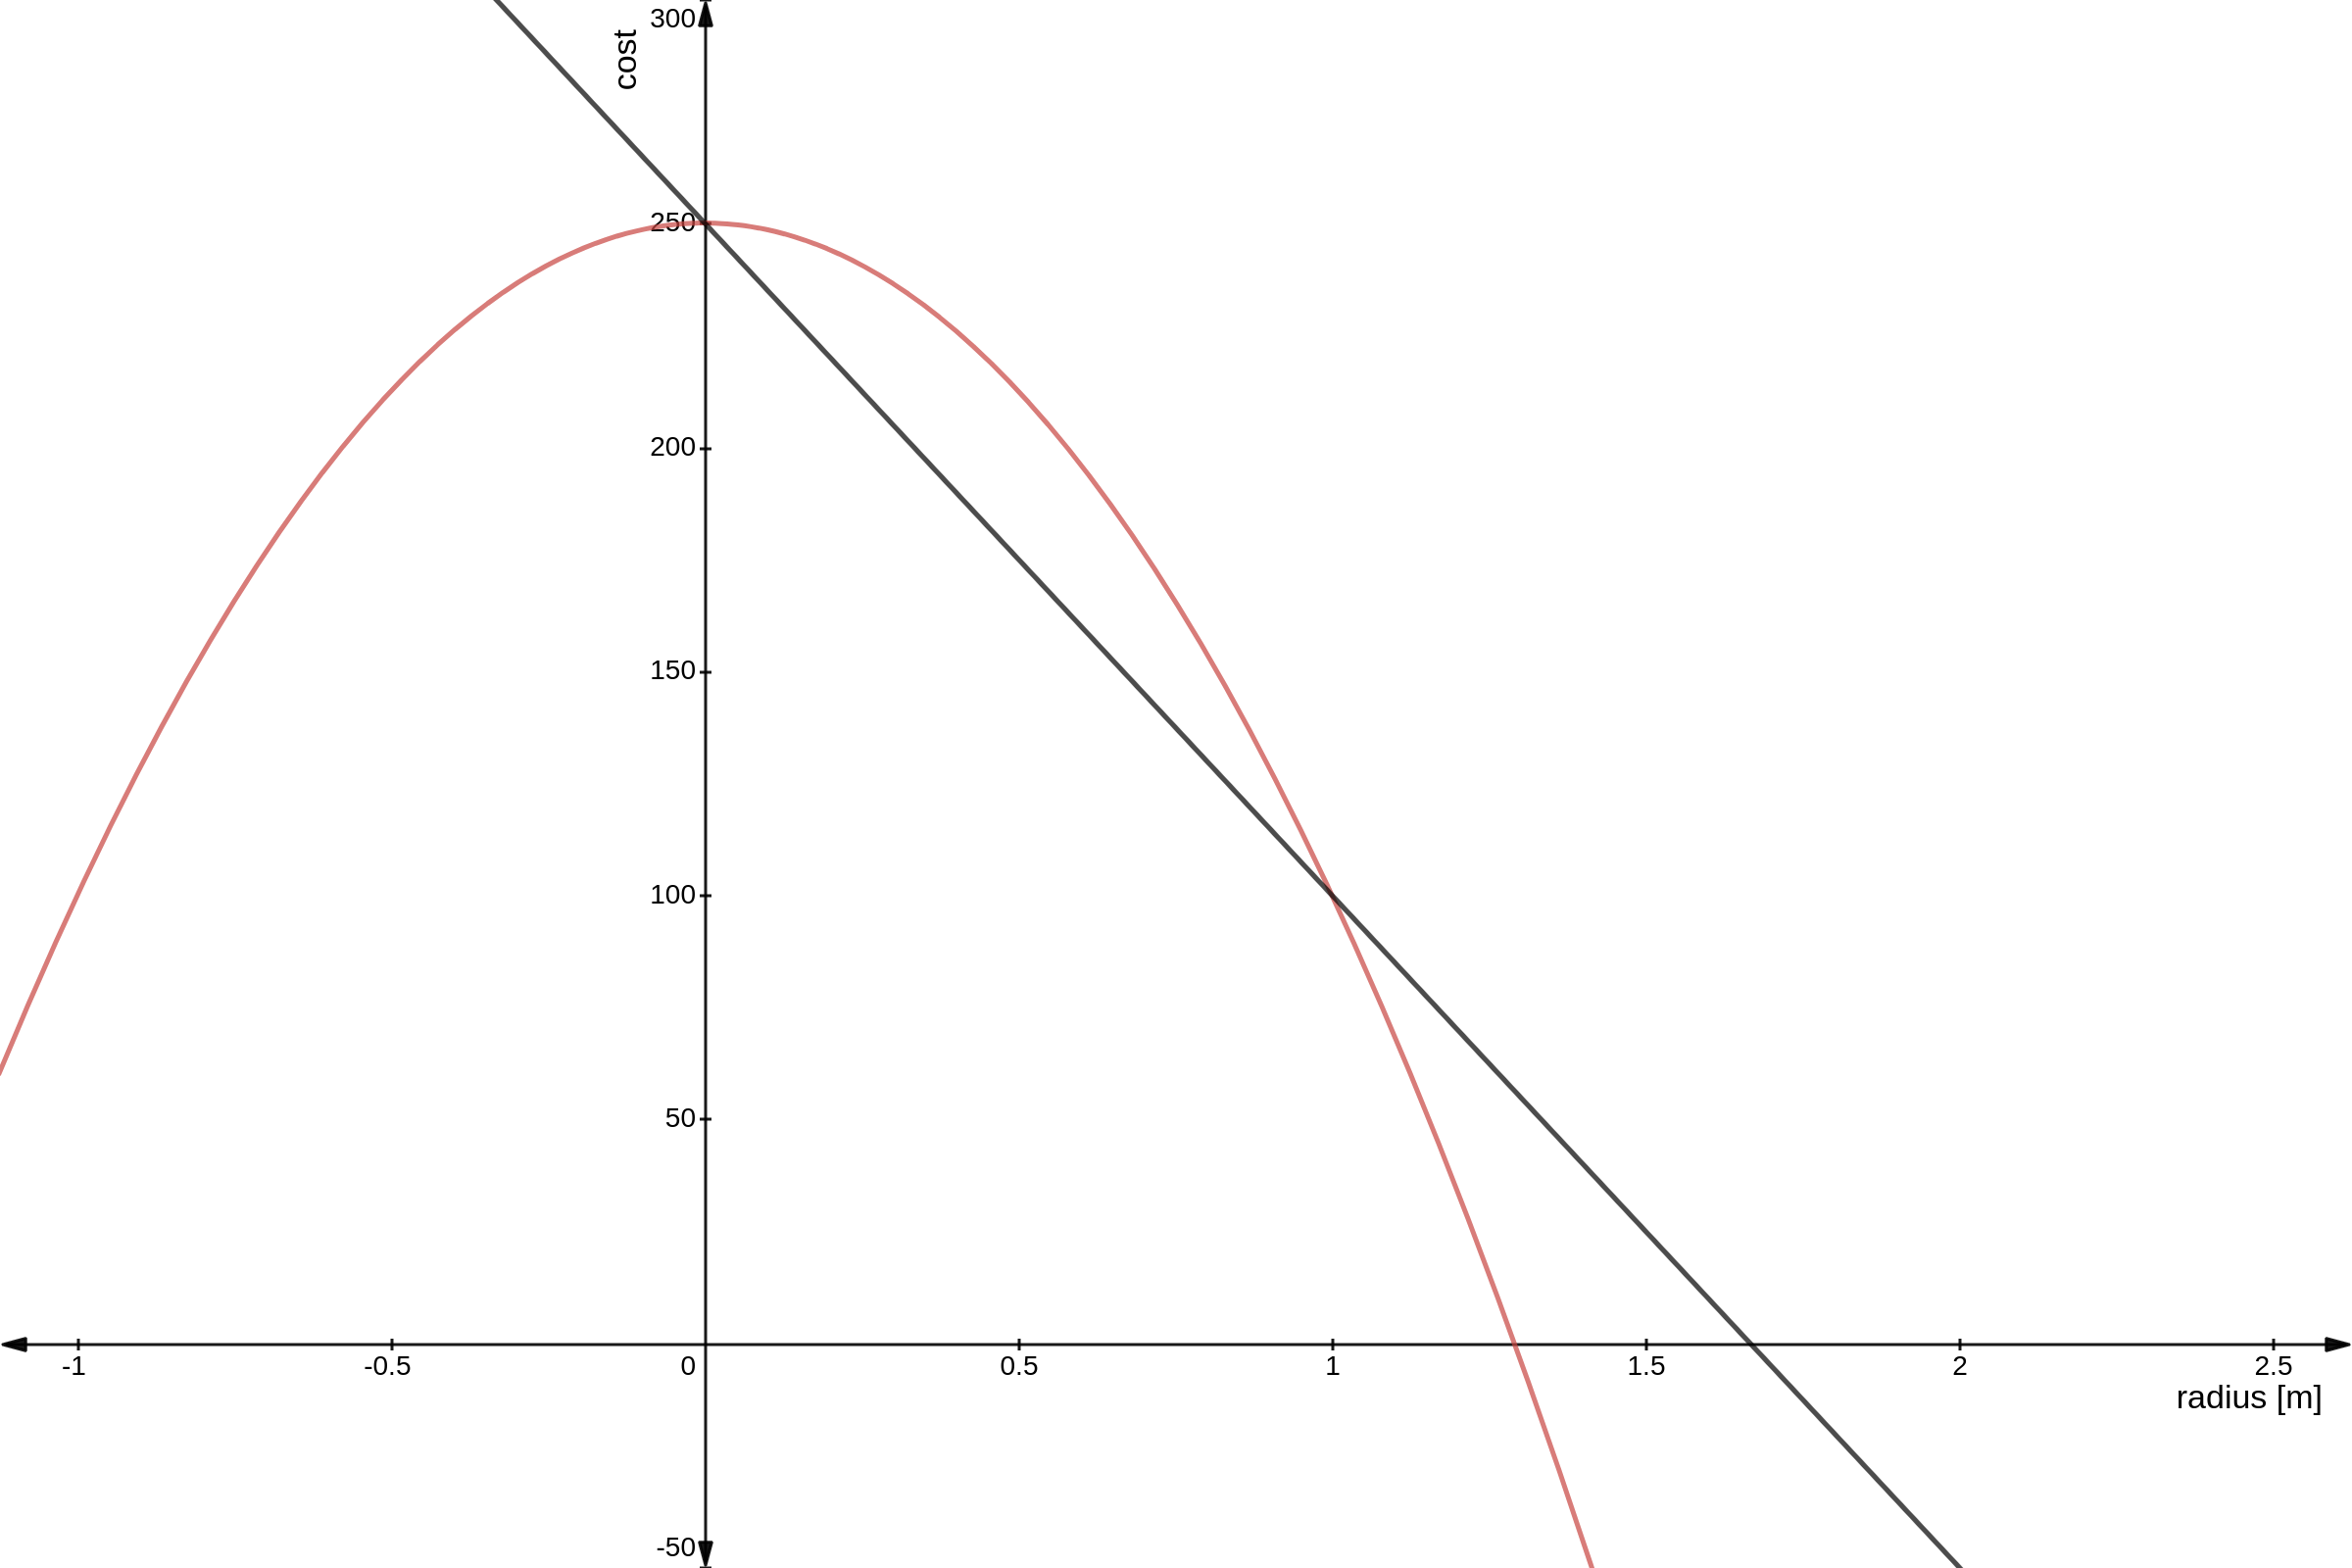
\includegraphics[width=140mm]{Pictures/linear cost comparison}
	\caption{cost distribution comparison with maxcost=250 mincost=100 radius=1}
	\end{center}
\end{figure}

When adding the inflation around points, the maximum of the calculated cost value and the current value of the cell in the costmap is set.
This leads to a problem, when trying to clear zones in the costmap, since then the minimum cost of the two needs to be set. Therefore setting zero as the cost value has the privileges for overwriting high cost values in the costmap.
 To prevent the cleared cells from being overwritten by the inflation of the next point, the clearing points have to be the last points in the input point cloud.\\

Figure \ref{dyncost} shows an avoidance of a simulated obstacle and the cost distribution in the costmap, generated by this layer. It is noticeable, that the right lane (in driving direction) has a clear zone over the entire length. Furthermore the cost around the points detected by the lidar have been removed.


\begin{figure}[H]
	\centering
	\begin{subfigure}{.45\linewidth}
		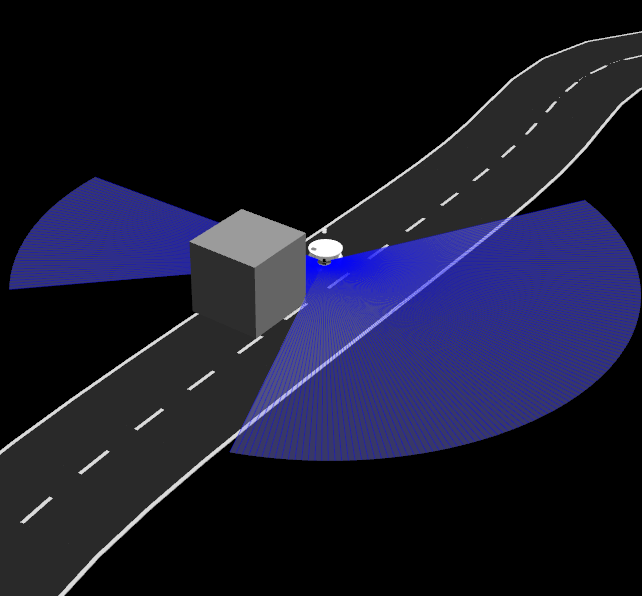
\includegraphics[width=\textwidth]{Pictures/avoidance}
		\caption{simulation environment}
		\end{subfigure}	
	%\hskip2em
	\begin{subfigure}{.45\linewidth}
		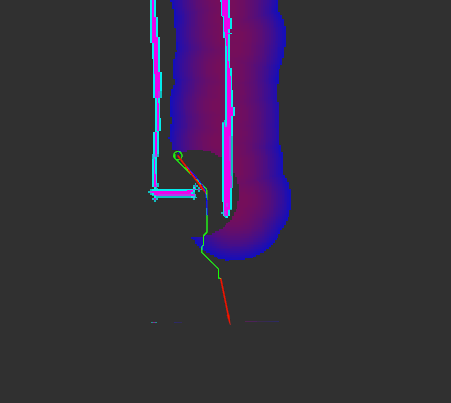
\includegraphics[width=\textwidth]{Pictures/avoid cost}
		\caption{costmap filled by the dynamic\_inflation\_layer}
	\end{subfigure}
	\caption{resulting cost during avoidance}
	\label{dyncost}
\end{figure}


The layer can be configured individually for the costmap using rqt\_reconfigure and the following parameters.




\begin{table}[H]
\centering
\resizebox{\columnwidth}{!}{%
	\begin{tabular}{ l l l }
	
 	\textbf{Parameter} & \textbf{Description} & \textbf{Range}\\
 	enabled & Whether to apply this plugin or not & [bool]\\
 	point\_topic & The Topic of the PointCloud containing Points and channel values for inflation radius & [string]\\

	\end{tabular}
}
\label{dynlayerparams}
\caption{dynamic\_cost\_layer parameters}
\end{table}




\section{MarkFreeSpace}

Like described in the concept, the purpose of this node is to provide data to the SLAM algorithm as well as to the costmaps. This data consists from the points on the polynomials of the road detection in combination with the filtered points of the lidar scan.\\
Based on the option of the obstacle\_layer of the costmap to raytrace marked obstacles, it needs to receive a PointCloud2 that contains points from the polynomials of the road detection. Raytracing the data removes the artifacts of previous measurements, as pictured in \ref{raytracing road}. 
This displays two measurements, that are slightly rotated based on noise. Like pictured, without raytracing this would lead to a restricted road width in the costmap.

When looking at the ray-traced version, it is noticeable, that the old left road marking has been removed, since the newest measurement is behind it. The right road marking has not been removed, since the old measurement is behind the new one.

This allows to handle the noise of the camera and the road detection, which otherwise could significantly hinder the navigation, especially in the very limited room on the road.

\begin{figure}[H]
	\centering
	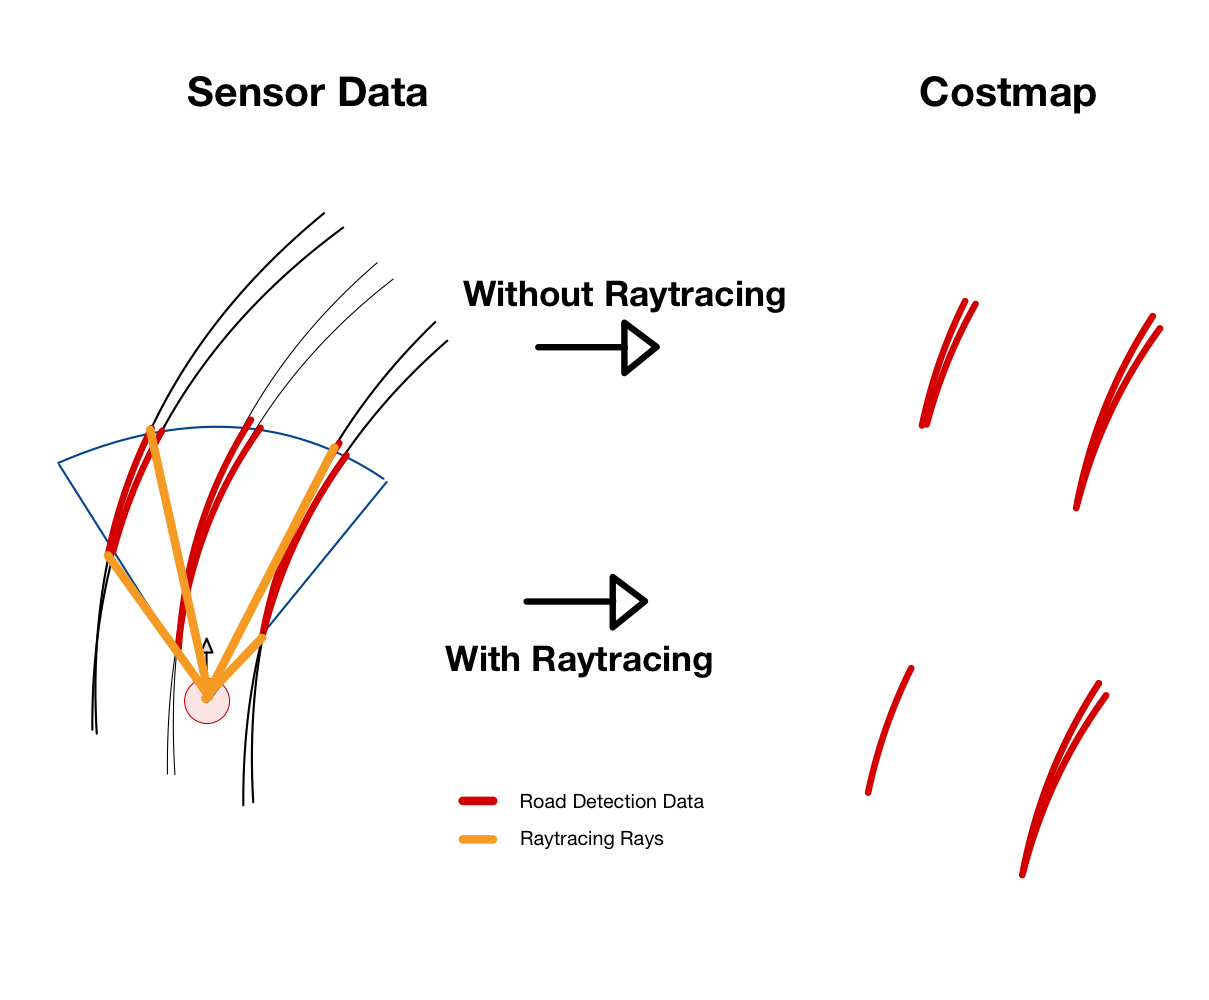
\includegraphics[width=.9\textwidth]{Pictures/raytracing road}
	\caption{raytracing of the road data}
	\label{raytracing}
\end{figure}

If this pointcloud would contain the points of the lidar as well, the obstacle layer would remove the points of the road marking, if an obstacle is behind it, as pictured in figure \ref{raytracing}.\\

\begin{figure}[H]
	\centering
	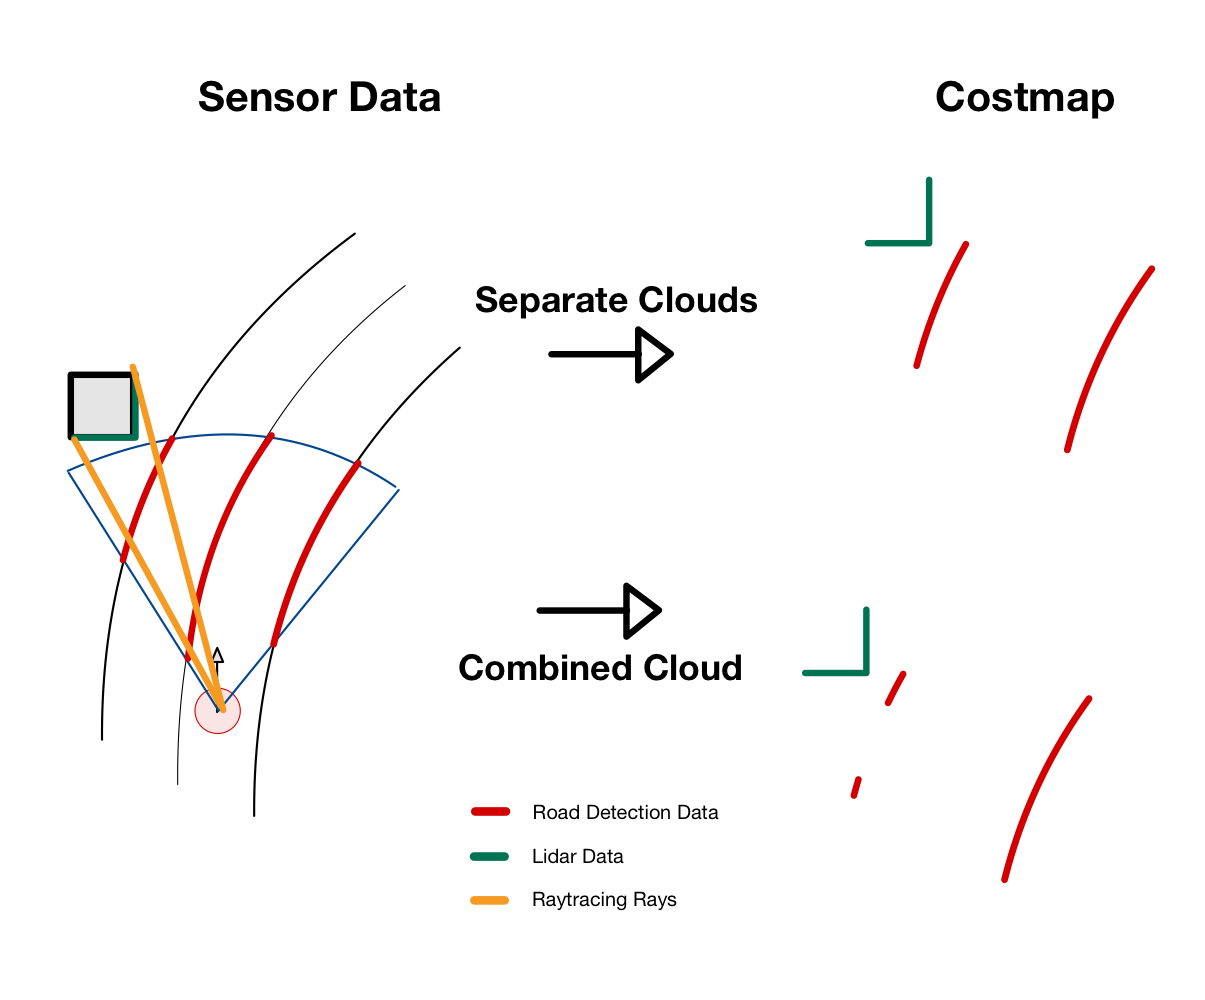
\includegraphics[width=.9\textwidth]{Pictures/raytracing}
	\caption{combined vs. separate point clouds during raytracing}
	\label{raytracing}
\end{figure}

For the SLAM algorithm both data sources need to be fused into one point cloud. Therefore, the points need to be transformed into the same frame and time, before being published.\\

The data for the developed dynamic\_cost\_layer has to contain more information. It is in the form of a point cloud and contains channel values for point individual inflation radius, min-cost and max-cost.\\ 

This pointcloud contains points of three types, left lane, right lane and obstacle.
The individual parameters for these points are pictured in \ref{markparams}. Using these parameters the cost distribution generated by the dynamic\_inflation\_layer can be modified.\\

\begin{figure}[H]
	\centering
	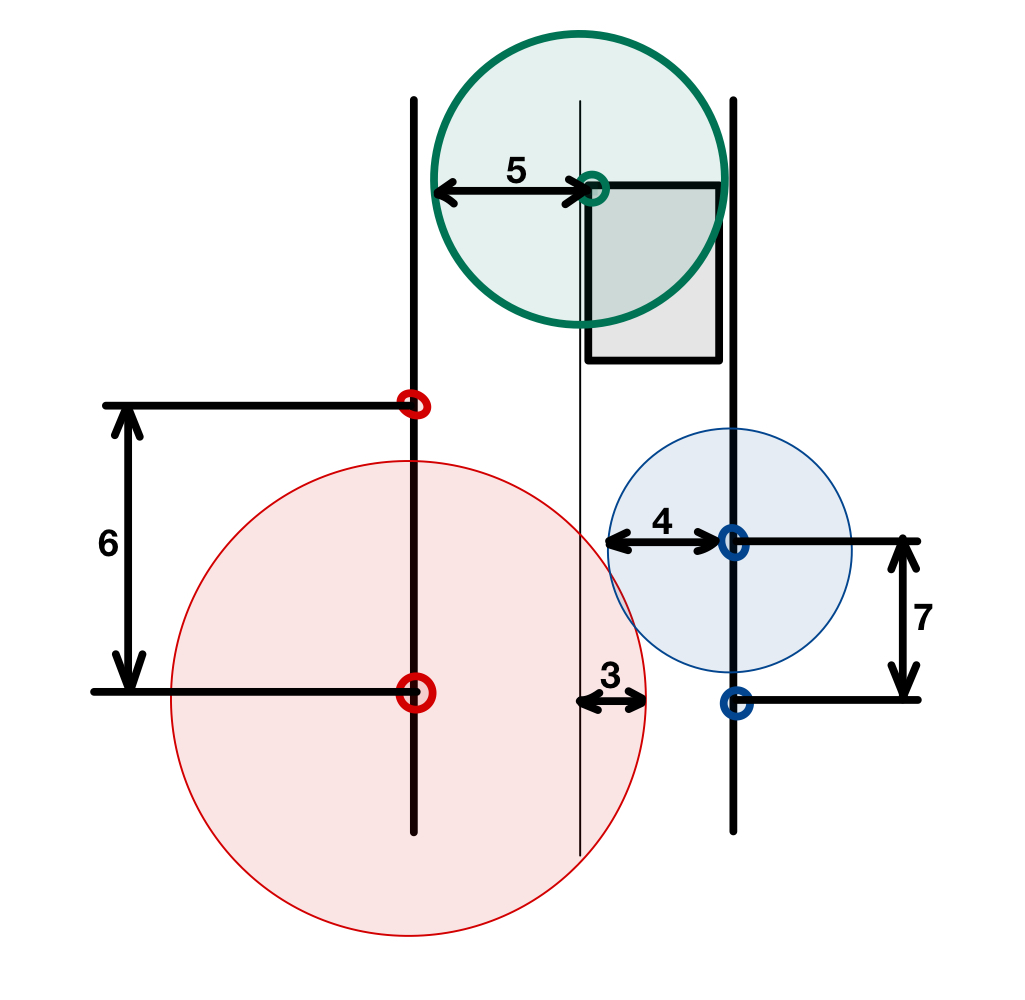
\includegraphics[width=.7\textwidth]{Pictures/markfreespace parameter erklaerung}
	\caption{top view of road with parameter}
	\label{markparams}
\end{figure}

The red points in the sketch represent the points of the left road marking. The distance between these points can be configured, in order to reduce the computational load on the dynamic\_cost\_layer. The same is possible for the blue points on the right road marking. Both points have a configurable radius, that is relative to the coverage of the right lane.\\
In addition to that the points of the left road marking receive max-cost and min-cost values for the required cost distribution. The points of the right road marking will only be used for the removal of costs.\\

The green point represents one of the measurements of the lidar sensor. Around this, the dynamic\_cost\_layer is supposed to generate a cost free zone, to improve path finding around obstacles.

The numbers in figure \ref{markparams} correspond to those of the following parameter list, that shows the specific names of all configurable parameters:

\begin{table}[H]
\centering
\resizebox{\columnwidth}{!}{%
\begin{tabular}{ l l l }
	
 \textbf{Parameter} & \textbf{Description} & \textbf{Range}\\
 maxCost & Maximum cost of the left lane inflation & 0-254\\ 
 minCost & Minimum cost of the left lane inflation & 0-254\\  
 leftInflation & How far the inflation of the left lane overlaps the right lane (3) & 0-1\\  
 rightRemoval & How much of the right lane will be cleared from cost (4) & 0-1\\  
 obstacleRemoval & Distance around obstacles on the road where no cost gets placed (5) & 0-2 [m]\\  
 inflPointDistance & min Distance between inflated points 0 for only last (6) & 0-5 [m]\\ 
 clearPointDistance & min Distance between points that clear cost 0 for only last (7) & 0-2 [m]\\   
\end{tabular}
}
\caption{MarkeFreeSpace parameters}
\label{markfreespaceparams}
\end{table}












\section{SLAM}
There are numerous lidar based SLAM packages available for ROS, but with the defined restriction of being able to use both, the points extracted from the road detection, as well as the lidar scan, most of the lidar based SLAM algorithms wont work since they only accept one lidar scan.\\
This rules out the popular options for lidar based SLAM like gmapping and HectorSLAM and the well documented package Google Cartographer will be used based on its flexibility in regards to robot configurations.\\
This package comes with an advantage of being based on loop closure, which might be useful when driving rounds in a circuit stile environment. The robot will drive the same route over and over again and thus the map could get more and more reliable over time even though the data is similar for different parts of the circuit and therefore not idal for the use with a SLAM algorithm.\\

Google Cartographer accepts numerous different input types including both point clouds and lidar scans. Additionally Google Cartographer can use provided odometry, as well as IMU data to improve the quality of the map.\\








